\documentclass{beamer}
%
% Choose how your presentation looks.
%
% For more themes, color themes and font themes, see:
% http://deic.uab.es/~iblanes/beamer_gallery/index_by_theme.html
%
\mode<presentation>
{
  \usetheme{Madrid}      % or try Darmstadt, Madrid, Warsaw, ...
  \usecolortheme{beaver} % or try albatross, beaver, crane, ...
  \usefonttheme{serif}  % or try serif, structurebold, ...
  \setbeamertemplate{navigation symbols}{}
  \setbeamertemplate{caption}[numbered]
} 

\usepackage{hyperref}
\usepackage{tabu}
\usepackage[italian]{babel}
\usepackage[utf8]{inputenc}
\usepackage{pdfpages}
\usepackage{framed, color}
\definecolor{shadecolor}{rgb}{1,0.8,0.3}
\usepackage{color}
\usepackage[backend=bibtex, style=numeric,sorting=none]{biblatex}

\definecolor{pblue}{rgb}{0.13,0.13,1}
\definecolor{pgreen}{rgb}{0,0.5,0}
\definecolor{pred}{rgb}{0.9,0,0}
\definecolor{pgrey}{rgb}{0.46,0.45,0.48}

\usepackage{listings}
\lstset{language=Python,
  showspaces=false,
  showtabs=false,
  breaklines=true,
  showstringspaces=false,
  breakatwhitespace=true,
  commentstyle=\color{pgreen},
  keywordstyle=\color{pblue},
  stringstyle=\color{pred},
  basicstyle=\ttfamily,
  frame=lrbt,xleftmargin=\fboxsep,xrightmargin=-\fboxsep
}

\title[Ragazze Digitali 2019]{Ragazze Digitali A.A. 2018/2019}
\author{E. Salvucci - S. Gattucci - C. Varini}
\date{}

\AtBeginSection[]
{
  \begin{frame}<beamer>
    \frametitle{Outline}
    \tableofcontents[currentsection,currentsubsection]
  \end{frame}
}

\bibstyle{unsrt}
\bibliography{bibliography.bib}

\begin{document}

\setbeamertemplate{background}
{
\includegraphics[width=\paperwidth,height=\paperheight]{images/ragazze_digitali.jpg}}
\begin{frame}
\end{frame}

\setbeamertemplate{background}{}

\begin{frame}{Cosa faremo oggi}
\texttt{Ti trovi in una terra piena di draghi.\newline
        Di fronte a te ci sono due grotte\newline
        In una grotta si trova un drago simpatico e socievole che condividerà con te il suo tesoro.\newline
        Nell'altra grotta c'è invece un drago affamato e vorace.\newline
        Dentro quale grotta vuoi entrare? (1 o 2)\newline}
\textbf{1\newline}
\texttt{Entri nella caverna 1\newline
        E' buia e spaventosa\newline
        Un enorme drago compare all'improvviso davanti a te! Apre le sue fauci e... ti inghiottisce in un batter d'occhio!\newline
        Vuoi giocare ancora?\newline}
\textbf{No}        
        
\end{frame}

\begin{frame}{Serviranno le funzioni di alcuni moduli}
    
Cosa dobbiamo fare per poter richiamare funzioni di un modulo/libreria? 
\begin{block}{random}
Utilizzeremo la funzione randint() che abbiamo già visto
\end{block}

\begin{block}{time}
Utilizzeremo la funzione sleep(forSeconds)
\end{block}

\end{frame}

\begin{frame}[fragile]
\frametitle{Il regno dei draghi - Codice}

    \begin{lstlisting}
        import random
        import time
    \end{lstlisting}

\end{frame}

\section{Funzioni}

\begin{frame}[fragile]
\frametitle{Funzioni}
    \begin{block}{}
        \begin{itemize}
            \item Abbiamo già visto e usato alcune funzioni, ad esempio: print('ciao'), input(), randint(1, 20), ecc..
            \item Possiamo anche crearne noi!
            \item Con le funzioni possiamo incapsulare del codice e riutilizzarlo più volte nel nostro programma.
        \end{itemize}
    \end{block}
    
    \begin{block}{Una funzione}
        \begin{itemize}
            \item Deve essere dichiarata \textbf{prima} di essere chiamata
            \item Può avere dei parametri
            \item Restituisce un risultato
        \end{itemize}
    \end{block}
\end{frame}

\begin{frame}[fragile]
\frametitle{Frame Title}
        \begin{block}{Come si dichiara una funzione}
            \begin{itemize}
                \item Utilizziamo la keyword \textbf{def}
                \item seguita dal \textbf{nome} della funzione
                \item Seguita dai \textbf{parametri} racchiusi tra parentesi (o le sole parentesi aperta e chiusa nel caso non ci siano parametri)
                \item Seguiti da \textbf{:}
            \end{itemize}
        \end{block}

        \begin{columns}
	    \begin{column}{4cm}
			\begin{figure}
   				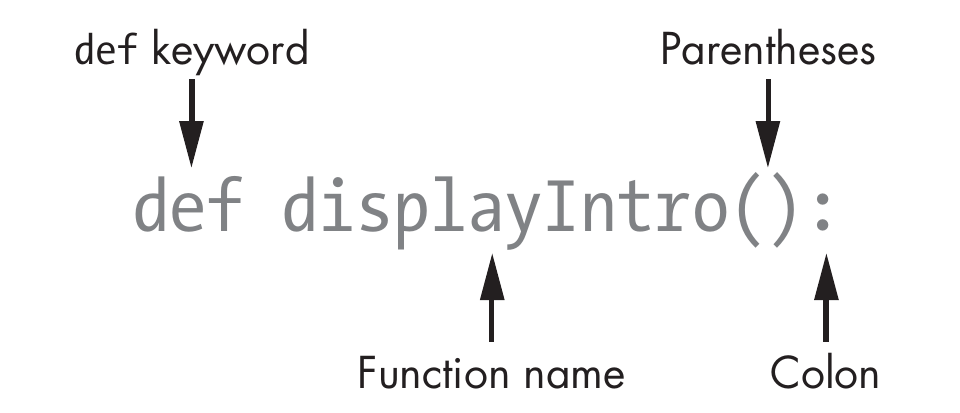
\includegraphics[height=2cm]{images/function_signature_example.png}
			\end{figure}
		\end{column}
		
		\begin{column}{6cm}
            \begin{lstlisting}
def displayIntro():
    print('''Ti trovi in una terra piena di draghi...''')
    print()
            \end{lstlisting}
		\end{column}
	\end{columns}
	! notiamo il print(''' '''), stringa multilinea
\end{frame}

\begin{frame}
\frametitle{Funzioni}
    \begin{block}{Alcuni consigli..}
        \begin{itemize}
            \item Ciò che abbiamo detto per i nomi delle variabili vale anche per i nomi delle funzioni
            \item Meglio se le nostre funzioni sono corte, con poco codice
            \item  Con 1 funzione facciamo 1 cosa soltanto!
            \item Evitiamo di usare più di 1 o 2 parametri in una funzione
            
            Se abbiamo bisogno di più parametri dividiamo quello che vogliamo fare in più funzioni
        \end{itemize}
    \end{block}
\end{frame}

\begin{frame}[fragile]
\frametitle{Funzioni}
    \begin{block}{Funzioni con parametri}
        \begin{itemize}
            \item Possiamo "dare in pasto" ad una funzione dei dati, delle informazioni, che chiamiamo \textbf{parametri}
            \item Queste informazioni ci serviranno per elaborare il risultato della funzione
        \end{itemize}
    \end{block}
    
    \begin{lstlisting}
                          # O ancora meglio..
def isPositive(number): | def isPositive(number): 
    if number > 0 :     |    return number > 0
        return True     |
    else:               |
        return False    |
    \end{lstlisting}
    
    \begin{lstlisting}
# Usiamo la funzione, ad esempio, in questo modo
print(isPositive(5))    # True
print(isPositive(-5))   # False
    \end{lstlisting}
    
\end{frame}

\begin{frame}[fragile]
\frametitle{Funzioni}
    \begin{block}{Funzioni con parametri}
        \begin{itemize}
            \item Possiamo "dare in pasto" ad una funzione dei dati, delle informazioni, che chiamiamo \textbf{parametri}
            \item Queste informazioni ci serviranno per elaborare il risultato della funzione
            \item Il risultato verrà restituito utilizzando la keyword \textbf{return}
        \end{itemize}
    \end{block}
    
    \begin{lstlisting}
def sum(firstNumber, secondNumber): 
    return firstNumber + secondNumber
    \end{lstlisting}
    
    \begin{lstlisting}
# Usiamo la funzione, ad esempio, in questo modo
result = sum(5, 4)    # result avra' valore 9
result = sum(-10, 5)  # result avra' valore -5
    \end{lstlisting}
    
\end{frame}

\section{Variabili locali e variabili globali}

\begin{frame}[fragile]
\frametitle{Variabili locali e variabili globali}
    \begin{block}{Variabili locali}
        Chiamiamo \textbf{Variabile locale} qualunque variabile dichiarata all'interno di una funzione, questa esiste solo all'interno della funzione stessa
        
        Le variabili locali vengono "dimenticate" dopo che la funzione ha raggiunto il return (e quindi ha finito le sue elaborazioni)
    \end{block}
    
    \begin{lstlisting}
def welcomePerson():
    person = 'Chiara'     # Variablile locale
    print('Benvenuta ' + person)
# Anche se non c'e' il return, da qui in poi la variable non ha piu' effetto
    \end{lstlisting}
    
    \begin{lstlisting}
welcomePerson()
person = 'Sofia'
print(person) # Sofia
welcomePerson() # Benvenuta Chiara
    \end{lstlisting}
\end{frame}

\begin{frame}[fragile]
\frametitle{Variabili globali}
    \begin{block}{Variabili globali}
        Nell'esempio precedente person = 'Sofia' e' una variabile globale, ovvero una variabile che ha effetto in tutto il nostro programma
        
        Modifichiamo leggermente l'esempio:
    \end{block}
    
        \begin{lstlisting}
def welcomePerson():
    print('Benvenuta ' + person)
    \end{lstlisting}
    
    \begin{lstlisting}
person = 'Chiara'     # Variablile globale
welcomePerson() # Benvenuta Chiara
person = 'Sofia'
welcomePerson() # Benvenuta Sofia
    \end{lstlisting}
\end{frame}

\section{Operatori booleani}

\begin{frame}[fragile]
\frametitle{Operatore and (e)}
\begin{block}{Quale frase è complessivamente vera e quale falsa?}
    \begin{itemize}
        \item I gatti hanno i baffi E i cani hanno la coda
        \item I gatti hanno i baffi E i cani hanno le ali
        \item I gatti abbaiano E i cani hanno le ali
    \end{itemize}
\end{block}

\end{frame}

\begin{frame}[fragile]
\frametitle{Operatore and (e)}

\begin{tabu} to 0.8\textwidth { | X[l] | X[c] | X[c] |  X[r] |}
 \hline
  & & & Risultato\\
 \hline
 True & \textbf{and} & True & True\\
 \hline
 True & \textbf{and} & False & False\\
 \hline
 False & \textbf{and} & True & False\\
\hline
 False & \textbf{and} & False& False\\
\hline
\end{tabu}

\end{frame}

\begin{frame}[fragile]
\frametitle{Operatore or (o)}
\begin{block}{Quale frase è complessivamente vera e quale falsa?}
    \begin{itemize}
        \item I gatti hanno i baffi O i cani hanno la coda
        \item I gatti hanno i baffi O i cani hanno le ali
        \item I gatti abbaiano O i cani hanno le ali
    \end{itemize}
\end{block}

    \begin{lstlisting}
city = 'Cesena'
result = 10 < 20 or city == 'Cesena'
# result avra' valore?
result = 10 > 20 or city == 'Cesena'
# result avra' valore?
    \end{lstlisting}

\end{frame}

\begin{frame}[fragile]
\frametitle{Operatore or (o)}

\begin{tabu} to 0.8\textwidth { | X[l] | X[c] | X[c] |  X[r] |}
 \hline
  & & & Risultato\\
 \hline
 True & \textbf{or} & True & True\\
 \hline
 True & \textbf{or} & False & True\\
 \hline
 False & \textbf{or} & True & True\\
\hline
 False & \textbf{or} & False& False\\
\hline
\end{tabu}

\end{frame}

\begin{frame}[fragile]
\frametitle{Operatore not}
    \begin{lstlisting}
city = 'Cesena'
result = not (10 < 20 or city == 'Cesena')
# result avra' valore?
result = not (10 > 20 or city == 'Cesena')
# result avra' valore?
    \end{lstlisting}

\end{frame}

\begin{frame}[fragile]
\frametitle{Operatore not}

\begin{tabu} to 0.8\textwidth { | X[c] |  X[c] |}
 \hline
  & Risultato\\
 \hline
 not True & False\\
 \hline
 not False & True\\
\hline
\end{tabu}

\end{frame}

\section{Costrutto while}

\begin{frame}[fragile]
\frametitle{Costrutto while}
\begin{block}{while}
    \begin{itemize}
        \item Costrutto simile al for, che abbiamo gia' visto
        \item Il while ripete il ciclo finche' una determinata condizone rimane vera 
        \item Qual e' la differenza con il for?
    \end{itemize}
\end{block}

    \begin{lstlisting}
while month == 'giugno' and year == '2019' :
    codice del ciclo while
    \end{lstlisting}
    
! come nel for, nell'if e nelle funzini occhio all'indentazione del codice del ciclo!

\end{frame}

\section{Il regno dei draghi}

\begin{frame}{Ritorniamo al gioco di oggi}
\texttt{Ti trovi in una terra piena di draghi.\newline
        Di fronte a te ci sono due grotte\newline
        In una grotta si trova un drago simpatico e socievole che condividerà con te il suo tesoro.\newline
        Nell'altra grotta c'è invece un drago affamato e vorace.\newline
        Dentro quale grotta vuoi entrare? (1 o 2)\newline}
\textbf{1\newline}
\texttt{Entri dentro la caverna 1\newline
        E' buia e spaventosa\newline
        Un enorme drago compare all'improvviso davanti a te! Apre le sue fauci e... ti inghiottisce in un batter d'occhio!\newline
        Vuoi giocare ancora?\newline}
\textbf{No}        
        
\end{frame}

\begin{frame}[fragile]
\frametitle{Il regno dei draghi - Parte 1}

\begin{block}{E' il vostro turno!}
Scrivi una funzione, chiamandola come preferisci, che stampi a video il testo introduttivo del gioco:\newline
        
        'Ti trovi in una terra piena di draghi.\newline
        Di fronte a te ci sono due grotte\newline
        In una grotta si trova un drago simpatico e socievole che condividerà con te il suo tesoro.\newline
        Nell'altra grotta c'è invece un drago affamato e vorace.\newline
        Dentro quale grotta vuoi entrare? (1 o 2)'
\end{block}

\end{frame}

\begin{frame}[fragile]
\frametitle{Il regno dei draghi - Parte 2}

\begin{block}{E' il vostro turno!}
Scrivi una funzione, chiamandola come preferisci, che chieda al giocatore di inserire il numero della grotta nella quale vuole entrare (1 o 2) e restituisca/ritorni il numero stesso della grotta scelta 

Aiuto:
\end{block}

    \begin{lstlisting}
answer = ''
while answer != '1' or answer != '2' :
    codice del ciclo while
    "ripensa al primo giorno quando chiedevamo all'utente il nome e stampavamo 'ciao nome'"
    \end{lstlisting}
\end{frame}

\begin{frame}[fragile]
\frametitle{Il regno dei draghi - Parte 3}

\begin{block}{E' il vostro turno!}
Scrivi una funzione, chiamandola come preferisci, che
    \begin{itemize}
        \item Prenda come parametro il numero della grotta scelto dal giocatore
        \item Stampi a video
            \begin{itemize}
                \item 'Ti avvicini alla grotta numero ...' (numero della grotta inserito dal giocatore 
                \item 'E' buia e spaventosa..'
                \item 'Un enorme drago compare all'improvviso davanti a te! Apre le sue fauci e...'
            \end{itemize}
        \item Dopo la stampa a video di ogni frase fai attendere 2 secondi al giocatore per aggiungere suspance utilizzando la funzione sleep del modulo time
    \end{itemize}
\end{block}

    \begin{lstlisting}
time.sleep(2) # Interrompe l'esecuzione del programma per i secondi specificati come parametro
    \end{lstlisting}
\end{frame}

\begin{frame}[fragile]
\frametitle{Il regno dei draghi - Parte 3}

\begin{block}{E' il vostro turno!}
Nella funzione della pagina precendete, dopo le stampe e i time.sleep(2)
    \begin{itemize}
        \item Aggiungi una variabile friendlyCave dandole un valore random tra 1 e 2 (utilizzando la funzione randint del modulo random come mostrato nel codice qui sotto)
        \item Se la variabile friendlyCave ha lo stesso valore del numero della grotta scelta dal giocatore allora stampa
        
        'Hai vinto il tesoro!'
        
        altrimenti stampa
        
        'Il drago ti mangia in un boccone!'
    \end{itemize}
\end{block}

    \begin{lstlisting}
friendlyCave = random.randint(1, 2)
    \end{lstlisting}
\end{frame}

\begin{frame}[fragile]
\frametitle{Il regno dei draghi - Parte 4}

\begin{block}{E' il vostro turno!}
Dopo aver inizializzato una variabile chiamata 'playAgain' con valore 'si', utilizza un ciclo while che si ripeta finche' il valore di playAgain e' la stringa 'si' e al suo interno
    \begin{itemize}
        \item Richiami la prima funzione che avete creato per stampare il testo introduttivo del gioco
        \item Crei una variabile locale con il valore della grotta scelta dal giocatore (richiamando la seconda funzione che avete creato)
        \item Controlli se il valore della grotta scelta sia lo stesso della friendlyCave (richiamando terza funzione che avete creato)
        \item Infine stampi a video la stringa 'Vuoi giocare ancora?' e riassegni/modifichi il valore della variabile playAgain con la nuova scelta del giocatore (usando la funzione input())
    \end{itemize}
\end{block}
\end{frame}

\end{document}



